\[
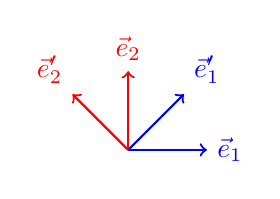
\begin{tikzpicture}[scale=0.5]
\coordinate (O) at (0,0);
\coordinate (X) at (2,0);
\coordinate (Y) at (0,2);
\coordinate (a) at (1.414,1.414);
\coordinate (b) at (-1.414,1.414);
\draw[->,thick,blue](O)--(X) node[pos=1,right] {$\vec{e}_1$};
\draw[->,thick,red](O)--(Y) node[pos=1,above] {$\vec{e}_2$};
\draw[->,thick,blue](O)--(a) node[pos=1,above right] {$\vec{e}'_1$};
\draw[->,thick,red](O)--(b) node[pos=1,above left] {$\vec{e}'_2$};
\end{tikzpicture}
\]